\ylDisplay{Tulehõõrumine} % Ülesande nimi
{Jaak Kikas} % Autor
{piirkonnavoor} % Voor
{2008} % Aasta
{G 3} % Ülesande nr.
{2} % Raskustase
{
% Teema: Termodünaamika
\ifStatement
Jõuga $F$ otsapidi vastu tasast pinda surutud toru pöörleb sagedusega $f$. Toru läbimõõt on $D$ ja seina paksus $d \ll D$. Toru otspind on risti toru teljega, hõõrdetegur toru ja tasapinna vahel on $\mu$. Kui palju soojusenergiat vabaneb ajavahemiku $\Delta t$ jooksul?

\begin{center}
	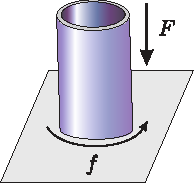
\includegraphics[width=0.3\linewidth]{2008-v2g-03-yl}
\end{center}
\fi


\ifHint
Varda pöörlemisel käigus muutub hõõrdejõu $F_h$ ületamiseks kulutatud töö soojuseks. Töö on leitav hõõrdejõu ja läbitud tee pikkuse korrutisena.
\fi


\ifSolution
Varda pöörlemisel käigus muutub hõõrdejõu ületamiseks tehtud töö soojuseks. Toru otspinna ja aluse vahel mõjub hõõrdejõud $F_h$, mis võrdub pinnaga ristuva rõhumisjõu ja hõõrdeteguri korrutisega. Rõhumisjõuks on jõud $F$, millega surutakse toru vastu alust. Seega $F_h = \mu F$. Kui toru teeb ühe pöörde, siis läbib toru sein teepikkuse $L = \pi D$. Hõõrdejõu ületamiseks tehti ühe pöörde läbimisel töö $A = F_hL$. Kui toru pöörleb sagedusega $f$, siis aja $t$ jooksul teeb toru $N = f t$ pööret. Kokku eraldub toru pöörlemisel soojushulk
\[
Q=A N=\mu F \pi D f \Delta t.
\]
\fi
}